\documentclass[11pt,letterpaper]{article}

\usepackage{amsfonts}
\usepackage{amsmath}
\usepackage{amssymb}
\usepackage[title]{appendix}
\usepackage{color}
\usepackage{csquotes}
\usepackage[margin=1in]{geometry}
\usepackage{graphicx}
\usepackage{multirow}
\usepackage{pifont}
\usepackage{tabularx}
    \newcolumntype{L}{>{\raggedright\arraybackslash}X}
\usepackage[usenames,dvipsnames,table]{xcolor}
\usepackage{xspace}
\usepackage{url}

\newcommand{\parhead}[1]{\medskip \noindent \textbf{#1}~~}
\newenvironment{widelist}{\begin{list}{$\bullet$}{\setlength{\leftmargin}{.40cm}\setlength{\itemsep}{.00cm} }}{\end{list}}
\newcommand{\cmark}{\ding{108}}
\newcommand{\xmark}{ }
\newcommand{\pmark}{\ding{109}}
\newcommand{\name}{Phoenix\xspace}
\newcommand{\Name}{Phoenix\xspace}

\title{Pisces}
\author{Stephen Herwig}
\date{July 2, 2019}
\begin{document}
\maketitle
\begin{abstract}

Organizations shift the deployment of their services to untrusted third
parties, such as cloud infrastructures, content delivery networks, or email
providers, in order to reduce costs, increase availability, or gain
additional protections inherent to these hosting environments.
%
Unfortunately, such a shift poses a security tradeoff: third-parties that
provide or host the application potentially gain access to sensitive
information about the organization or its clients.


In my proposal, I ask whether it is possible to run legacy application binaries
with confidentiality and integrity guarantees that reflect the
organization's trust model with respect to the application and its
deployment setting.
%
The constraint of running unmodified, legacy applications implies that the
enforcement of such guarantees is the responsibilty of the applications's
run-time execution environment. 
%
Since the execution environment is transparent to the application, the insight
is that it may be modified, partitioned, and distributed across domains of
varying trustworthiness, so as to reflect the security goals.


In the first part of my proposal, I review my prior work in extending a
library operating system that runs within an Intel SGX secure hardware
enclave, so as to support running a broader set of trusted, legacy,
applications in untrusted environments.
%
In the second part, I propose a new run-time system, \emph{Gemini}, that is
agnostic to the availability of secure hardware and the trustworthiness of
the application.
%
Gemini presents two complementary abstractions: \emph{distributed containers},
where organizations pin sensitive data to domains that they trust, and
\emph{policy monitors}---modules that an organization installs in a trusted
environment to enforce expected behavior of untrusted applications.
%
I present the design of Gemini and propose a set of evaluations for assessing
its correctness and performance.

\end{abstract}

\section{Introduction}
\label{sec:intro}

Software is often written assuming monolithic trust assumptions, meaning that
the user tacitly trusts both the software and the environment in which it runs.
%
This assumption worked fine in the past, when an organization developed the
software, owned the infrastucture, and administered all parts of the resultant
system.
%
However, the trust assumption must be updated as new deployment scenarios bcome available.
%
A prime example is an organizations that outsources its services to untrusted
third parties, such as content delivery networks and mail providers.
%
Outsourcing is an attractive way for an organization to to reduce costs,
increase availabilty, or gain additional protections inherent to these hosting
environments.
%
Unfortunately, such a deployment poses a security tradeoff: the third party
providers that offer or deploy these services potentially gain access to
sensitive information about the organization and its clients, and the
organization may no longer have insight into what specific software is
implementing the service.


% TODO: maybe expand this paragraph a bit
%
% XXX: the problem is larger than just running trusted software on an untrusted
% host.
Running applications with strong security and privacy guarantees on untrusted
third parties is a large and active area of research; it spans uses of
trusted hardware and functional encryption that seek to continue hosting
applications completely on third parties, to (re-)designing applications and
protocols so as to delegate trust, preserve privacy, or otherwise partition
the application's execution across trust boundaries.
%
Unfortunately, this prior work either requires modifications to the
application, or has severe limits on the types of unmodified applications
supported.


% this is too specific
My thesis is:
\begin{displayquote}
    It is possible to run legacy application binaries with confidentiality and
    integrity guarantees that reflect the trust model in which the application
    is deployed.
\end{displayquote}
% Running unmodified, legacy binaries that have monolithic trust assumptions in
% environments where such assumptions do not hold.  

% For instance, an organization to outsource their unmodified, legacy, services
% to an untrusted hosting provider, who may in fact provide the service itself,
% without leaking private data to the provider and with guarantees that the
% provider does not deviate from the service's expected behavior.

The constraint of running unmodified, legacy services implies that the
enforcement of such security, privacy, and correctness guarantees is the
responsibilty of the service's run-time execution environment. 
%
Since the execution environment is transparent to the application, the insight
is that it may be modified, partitioned, and distributed across domains of
varying trustworthiness, so as to reflect the security goals of the
organization.


The design space is influenced by two factors: the presence of trusted
hardware, and the organization's trust in the application.
%
% Untrusted means the application may deviate arbitrarily from its stated
% purpose, subject to standard cryptographic assumptions, and, in particular, may
% actively try to leak sensitive data.
%
In my preliminary work, conclaves, I assume the presence of Intel SGX hardware
enclaves and that the content owners trust the service.
%
Conclaves extends prior work on SGX-based library operating systems (libOS) by
modifying a libOS to support running a broader set of legacy services
within enclaves: namely, multi-process, shared resource, applications.
%
% Specifically, conclaves is distributed system reminiscent of a microkernel,
% where each kernel service (for instance, a filesystem or shared memory)
% runs in a separate enclave and mediates the service’s shared resources
% among the application’s processes.


My proposed work, Gemini, makes assumptions about the availability of trusted
hardware and the trustworthiness of the application into policy specifications
on the part of the organization.
%
Gemini is an execution environment that offers two complementary abstractions:
(1) \emph{distributed container}, where organizations may pin sensitive data to hosts
that they trust; a thread's exeuction migrates to the trusted host when
computing with the sensitive data or any sensitive data derived from it, and
(2) \emph{policy monitors}, which are modules that an organization may installed in a
trusted environment that enforce expected behavior of untrusted application.
%
A key feature of policy monitors is that the policies enforce fine-grain
information flows.


To demonstrate this thesis, I make the following contributions:

This proposal is organized as follows:

% I evaluate my work by demonstrating correctness, measuring performance
% overheads, and measuring the “closeness” of the emergent protocols to proposed
% alternatives. I focus on the use cases of deploying TLS-enabled web services on
% content delivery networks (CDNs) without granting the CDN operator the private
% TLS key, as well as running database applications on untrusted third parties
% while maintaining the privacy of the database content.


% The conclaves
% paper is my "prior" work for this thesis, and the new work deals with migrating
% processes across trust domains (the unfinished work of a previous graduate
% student).




\section{Background}
\label{sec:background}

In this section, I clarify the problem with specific examples, and specifically
focuse on the everday case of outsourcing.
%
%
In this setting there are two principals: the \emph{organization} and the
\emph{cloud service provider}.
%
I describe the security and privacy implications of naively outsourcing, as
well as several trust models that apply to this setting, 
%
I then enumerate a list of goals for a system designed to handled these
implications.


\subsection{Problem}

There are two broad approaches of outsourcing.
%
The first, \emph{cloud hosting}, is an organization migrating its in-house
services to a third-party deployment; the second is an organization  migrating
from in-house services to those offered by third party \emph{cloud services}.
%
Hybrid approaches exist, such as where a cloud service provider must
communicate with the organization's, in-house, backend services.
%
Common outsourcing examples are an organization moving its HTTPS, DNS, or
email servers into the cloud, or contracting some other party to run its own
implementations of these services on the organization's behalf.
%
Nowadays, all of these core application-level protocols use public key
cryptography to ensure the integrity, authenticity, and/or confidentiality of
the application's content.


As a concrete example, consider an organization that outsources its web hosting
to a a content delivery network (CDN)\@.
%
A CDN is a massive, global network of \emph{edge servers}, where each edge
server acts as a reverse proxy for the organization: to
handle client requests, edge servers retrieve content from the organization's
\emph{origin servers}, and cache it so they can deliver it locally.
%
CDNs derive much of their utility from the fact that they have servers close to
most clients, thereby providing low-latency responses.
%
Several techniques exist for routing clients to the closest edge server, but
DNS is common, and so the CDN may also handle the organization's DNS server.
%
CDNs also provide added security benefits, such as absorbing DDoS
traffic, and filtering targeted malicious trafic, such as SQL injection and
cross-site scripting attacks~\cite{securing-cdns}.
%
Virtually all of the most popular websites (and a very long tail of unpopular
websites) use one or more CDNs to help reliably host their content.


With these use-cases in mind, let's enumerate the security and privacy
implications of outsourcing such service such services.


% XXX: try to keep each implication to one meaty paragraph.
\parhead{Impersonation}
% byzantine
%
In order for the provider to fulfill the service, the provider must
have access to the application's private keys.
%
Indeed, as the web moves towards HTTPS-everywhere~\cite{felt-2017-https},
organizations increasingly rely on CDN providers to store their HTTPS
certificate and the corresponding secret keys~\cite{key-sharing,
when-https-meets-cdn}, so that they can accept TLS connections while
maintaining low latency to clients.
%
Even with an application like DNS, where an organization would traditionally sign
its DNS records offline, the organization may choose to outsource the keys
and management to the provider.
%
% TODO: cite cloudflare blog
With the organization's private DNS keys online, the provider can offer
additional services, such as greater flexibility to return geographically-based
responses, as well as zone enumeration defenses.
%
This has significant implications on the trust model of each PKI and the web
writ large: today's providers can arbitrarily impersonate any of their customer
organizations.


\parhead{Breach of Confidentiality}
% Honest but curious
%
With the provider acting as a man-in-the-middle between the
organization and its clients, the provider is privy to the client's private
data, such as passwords, cookies, and personal content, as well as metadata 
for client profiling.
%
The provider might further subcontract aspects of the deployment (as with an
email provider using another provider for virus and spam scanning), with
the client and organization unaware of the extent of their data exposure.


\parhead{Correctness}
% concern 4: correctess: e.g., DNSSEC providers not actually providing DNSSEC.
% Negligent (also, a supertet of the byzantine and honest but curious)
%
By outsourcing a service, the organization no longer has guarantees that the
provider adheres to the expected service.
%
For instance, one DNS study~\cite{chung-2017-dnssec} discovered that 31\% of
domains that claim to support DNSSEC fail to publish all relevant records
required for a client resolver to validate the response, while
a study~\cite{open-http-proxies} of open HTTP proxies found that 5\% perform
unwanted or malicious content modification.


% TODO: call this something else
\parhead{Latent Trust Assumptions}
%
Assume a hybrid deployment where the organization has migrated its front-end
business applications to a cloud service provider, but that the application's
database remains within the organization’s network. 
%
Before migrating to the cloud, the database could trust that any connections to
it were from benign, internal tools; in the new deployment setting, the
organization must guard against potentially malicious or devious queries from
the cloud front-end.


\parhead{Legal and Regulatory Restrictions}
% concern 5: legal, policy compliance, ...restrictions
% talk about akamai not hosting content on thrid parties.
% talk about HIPPA (as with emails)
%
By outsourcing a service, the organization may be non-compliant with
industry regulations.
%
For instance, a hospital may be unable to run its electronic medical records
system in the cloud due to concerns  of HIPPA compliance.
%
In other words, even if the organization itself accepts the security and
privacy implications of outsourcing their services, legal matters may restrict
the degree to which the organization can leverage such deployments.


\subsection{Trust Model}

\begin{table}[t]
%\resizebox{.5\textwidth}{!}{
\small
\centering
\rowcolors{2}{gray!15}{white}
    \begin{tabular}{@{}lcccl@{}}
        & \textbf{Enclave}& \textbf{Provider} & \textbf{Software} & \textbf{Deployment} \\
        \hline
        1 & \cmark          &                   & \cmark          & Conclaves   \\
        2 &                 &                   & \cmark          & Gemini      \\
        3 & \cmark          &                   &                 & out of luck \\ % sandbox in enclave
        4 &                 &                   &                 & out of luck \\ % sandbox in partition
\end{tabular}
%}
\caption{The deployment strategy, depending on whether the provider offers
    trusted enclaves, whether the organization trusts the service provider, and
    whether the organization trusts the provider's application software.
    }
\label{tab:trust-models}
\end{table}

We describe an idealized trust model from the perspective of an
organization that uses a cloud service provider that requires the organization's
sensitive data.
%
For simplicity, we assume that the provider and the cloud machine owner are the
same party, and that the provider administers all software on the machine,
including any system software, such as the operating system, as well as the
application.
%
An untrusted provider may deviate arbitrarily from the stated service, but
remains subject to standard cryptographic assumptions.
%
Likewise, untrusted software may deviate abitrarily from its stated purpose
and, in particular, may actively try to leak sensitive data.
%
We assume, however, that the software is bug-free, and thus the model omits
external actors, such as a remote attacker.
%
The application may be composed entirely of open-source components, private
components that are proprietary to the provider, or some combination thereof.
%
If trusted boot is available  (either via a TPM, or in the form of secure
enclave launch), we assume that the organization and provider can agree to run
a specific build of system software, and that such software is trusted and
bug-free.


Table~\ref{tab:trust-models}, shows the different possible trust models based
on whether the provider offers hardware enclaves, whether the organization
trusts the provider, and whether the organization trusts the provider's
software.
%
We omit the uninteresting cases with a trusted provider, with the assumption
that the organization transitively trusts applications that the provider
offers.


In model 1, the organization trusts the software, but does not trust the
provider to run it faithfully, and thus uses one of various
approaches~\cite{talos,haven,scone,graphene} to
run an unmodified legacy application in an enclave.
%
This is the trust model for my prior work, conclaves, described in
\S\ref{sec:conclaves-summary}.
%
In contrast, in model 2, an enclave is not available (or assumed vulnerable to
to side-channnel attacks).
%
This is the starting use-case for Gemini, described in \S\ref{sec:gemini-design}.
%
In models 3 and 4, where neither the provider nor the software is trusted, no
general purpose solution exists for an organization to securely use an
commodity applicatins.


%For instance, the application may be composed of several components, some of
%which are trusted, and some are not; we assume that the organization
%trusts the components that interact with the senstive data.

In practice, the model's binary characterization of ``trusted" is too coarse,
the definition of untrusted as ``arbitrarily malicious" too strong,
and the assumptions of bug-free code and attacker-free environments too
naive.
%
For instance, it may be the case that most of the application is untrusted, but
the organization trusts a small portion of the application, such as its
cryptographic library.
%
This scenario is between models 2 and models 3 and 4, as the organization can
identify a small trusted computing base within the application.
%
Moreover, in the presence of attackers, an organization may simply
want strong, physical, isolation of its sensitive data from a remote attacker.
%
In other words, trust is a spectrum; the model highlights the endpoints of the
spectrums; my systems (conclaves and Gemini) target a specific endpoint, but,
to varying degress, allow for the relaxation of assumptions.



\subsection{Goals}

Our high-level goal is to allow the user to specify a trust policy to the
runtime execution environment; the runtime transparently implements the
policy on behalf of the applications.
%
I break down the policies into two categories:

\begin{widelist}
\item \textbf{Confidentiality policies:} Specifications of isolation boundaries for
    sensitive resources; the run-time constructs and enforces the boundaries.

\item \textbf{Integrity policies:} Specifications for data integrity; the run-time
    provides mechanisms for measuring integrity and detects breachs of
    integrity.
\end{widelist}


Our primary constraint is that the runtime should not require applications to be
rewritten or recompiled.
%
This is a practical constraint for system adoption, but also underscores our
thesis that such policies are deployment-specific, may be unknown during the
application's development, and must handle ``black box" applications, where the
source code is unavailable.
%
Our secondary constraint is that the policies should be simple; I want to avoid
degenerate solutions where the specification of the policy is more
onerous than simply rewriting the application.

Additional practical constraints, with respect to outsourcing, is that the policies
and runtime should handle applications that multiplex services across organizations,
with strong isolation between the organizations.
%
The system should also avoid degenerate solutions
that transfer undue hosting responsbilities back to the organization, thereby
defeating the intent of outsourcing.


Intuitively, the system will have worse performance than its vanilla
counterpart.
%
Nevertheless, the system should allow introspection into performance bottlenecks
as a means of investigating possible optimizations.


As non-goals, we are not concerned with obliviousness of the access paterns,
which may be a side-channel vector.

\section{Related Work}
\label{sec:related}

We present an overview of trusted execution environments, and then describe
three, not necessarily orthogonal techniques, for post-hoc adapting existing
software to satisfy alternative trust assumptions. 


\subsection{Trusted Execution Environments}

Trusted execution environments (TEEs) provide hardware protections for running
trusted portions of code with guarantees of confidentiality and integrity.  
%
Applications can be guaranteed that code executed within the TEE was run
correctly and that any secrets generated during execution will remain safely
within it as well.
%
A wide range of TEEs are available today, with varying functionalities.
%
We focus on Intel's Software Guard Extensions (SGX)\@.


\parhead{Intel SGX Overview}
%
Intel's SGX provides a new mechanism for trusted
hardware and software as an extension to the x86 instruction set~\cite{sgx,
mckeen2013innovative}.  
%
A program called an \textit{enclave} runs at high
privilege in isolation on the processor in order to provide trusted code
execution, while an untrusted application can make calls into the enclave.
%
While these enclaves can be statically disassembled (so the code running in the
enclave is not private), once an enclave is running, its internal state is
opaque to any observer (even one with physical access), as are any secrets generated.  


Enclaves must be measured and signed by their creator and cannot run without
this signature, and the enclave state is checked against this measurement
before running.  
%
An enclave can also cryptographically \textit{attest} to its current state, in
order to prove that it correctly executed code \cite{sgx_provisioning,
anati2013innovative}.  
%
Another feature is the ability to cryptographically \textit{seal} data to be
used across multiple invocations of an enclave~\cite{anati2013innovative,
sgx_sealing}.  
%
SGX also provides such features as trusted time and monotonic counters
\cite{sgx-linux-sdk,sgx-trusted-time}.  
%
However, as enclave code is always executed in user mode, system calls
must be proxied through the untrusted OS.


\parhead{AMD-SEV Overview}
%
%Whereas Intel SGX guards fine-grained units of execution, AMD's Secure
%Encryped Virtualization (SEV) is roughly the equivalent of an enclaved
%virtual machine.
%%
%SEV is based upon AMD Memory Encryption Technology, which introduces an
%AES-128 encryption engine inside the System on Chip (SoC) that transparently
%encrypts and decrypts the data when it leaves or enters the SoC, respectively.
%%
%Encryption key management, such as generating, storing, and delivering the
%keys, are carried out by the AMD secure processor and the encryption keys are kept
%hidden from untrusted parts of the platform.
%%
%The secure processor provides a set of APIs for provisioning and managing the
%platform in the cloud.
%
%
%SEV allows individual VMs to encrypt their memroy pages using their own secure
%keys; the VM's memory space is thus protected from from the hypervisor and
%co-resident VMs.
%%
%When code and data arrive into the SoC, SEV tags all of the code and data
%associated with the guest VM in the cache and limits access only to the tag's
%owner VM.
%%
%The guest OS is able to specify which memory pages are encrypted through new
%page table attributes.


\parhead{Attacks}
%
We must address the recent rise of side-channel attacks against SGX, including
the speculative execution attack Foreshadow~\cite{foreshadow,
weisse2018foreshadow}.  
%
This attack allows for the extraction of not only the entire SGX enclave's
memory contents but also the attestation and sealing keys.  
%
We note that this attack would break the security guarantees that we provide
with conclaves.
%
Intel has stated that SGX is explicitly designed to not deal with side-channel
attacks in its current state and leaves handling this up to enclave
developers~\cite{sgx-sidechannel, sgx-developers}.
%
Regardless, Intel has released both microcode patches and recommendations for
system level code that at the current time address Foreshadow and known related
attacks \cite{sgx-patch, canella2018systematic, weisse2018foreshadow}.  
%
There is also ongoing research to address both speculative execution as well as
other cache-based side-channel attacks on SGX and in general
\cite{yan2018invisispec, oleksenko2018varys, canella2018systematic, shih2017t}.

% TODO: add paragraph or two about attacks on SEV.


% Each solution operates at a differnet level in the stack, more or less.
% Handle TEE and non-TEE based solutions together.

\subsection{Partitioning applications across trust domains} 
% here, you can talk about program partitioning, both those that are aware of
% TEEs, and those that came before.


\parhead{Compiler Techniques}
%
Privtrans~\cite{privtrans} partitions a single program into two parts: a
privileged program called the monitor and an unprivileged program called the
slave. 
%
The monitor and slave run as separate processes, but communicate and cooperate
to perform the same function as the original program.
%
This is process-level isolation, and the monitor can be seen as interposing
between privileged operations and the main execution in the slave.


Privtrans allows a developer to add privilege separation to source code via
source-level annotations of variable and functions to indicate privileged
operations.  
%
Privtrans then propagates attributes, performs static analysis to find
privileged call sites, and performs C-to-C translation to partition the input
source code into the source code for the monitor and slave. 
%
Monitor must mediate access to all privileged resources, including the data
derived from such a resource; it is not sufficient for the monitor to only
perform access control.
%
In contrast, developers can augment monitors with application-specific
downgrade policies to make otherwise priviledged data flow from the monitor to
the slaves.  


\parhead{Protocol Refactoring}
%
Other work allows the organization to retain ownership of its private keys by
changing the server-side implementation of TLS\@.
%
SSL Splitting~\cite{ssl-splitting} leverages the fact that a TLS stream
comprises data records and authentication records (MACs), and develops a new
protocol in which the organization sends the authentication records and the
provider merges them with the data records to form the complete TLS stream.
%
Cloudflare's Keyless SSL~\cite{keyless-ssl} takes advantage of the fact that
TLS only uses the website's private key in a single step of the TLS handshake.
%
Like SSL Splitting, Keyless SSL keeps the master private key off of, and unknown
to, the proxy, but unlike SSL Splitting, Keyless SSL does not provide for
content provider endorsement of the content the proxy serves.  
%
Neither SSL splitting nor Keyless SSL provides for the protection of the
session keys from the provider.


\parhead{Virtualization Techniques} 
%
Several works~\cite{overshadow,inktag} that predate Intel SGX and AMD-SEV
extend the isolation capabilties of a hypervisor to give storng safety
guarantees to applications even in the presence of malicious guest operating
system.
%
These systems prevent the guest operating system from reading or modifying
application code, data, and registers through a technique called
\emph{cloaking}, in which the application sees a normal view of its memory
pages, but the OS an encrypted view.
%
Cloaking allows resources to remain accessible to the OS, yet secure,
permitting the OS to manage resources without compromising application
privacy or integrity.
%
Inktag also enables the hypervisor to verify the behavior of the untrusted
commodity operating system, as by checking that the memory mappings requested
by the application match those returned by the OS.


\subsection{Running (trusted) legacy applications in TEEs}
%
Various works use SGX as a mechanism for achieving shielded execution of
unmodified, trusted, legacy applications.
%
These works generally differ in how much of the application's code runs
within the enclave.


\parhead{Minimal TCB approachs}
%
At one extreme, TaLoS~\cite{talos} simply ports the LibreSSL library to SGX so
that the application terminates TLS connections in an enclave; the rest of
the application remains outside the enclave, unchanged.
%
% emphasize: smaller TCB, 
Several works~\cite{glamdring, panoply} generalize this approach by using developer
provided source-level annotations to partition an application into sensitive and
non-sensitive commponts, with the sensitive components running in an enclave.
%
In particular, Glamdring~\cite{glamdring} takes a similar approach to
Privtans~\cite{privtrans}, while also aiding a backslicing technique so that
fucntions and variables that influence a sensitive output are also isolated to
an enclave.  
%
Panoply~\cite{panoply} focuses less on the  partitioning scheme, but instead
allows the application to be partitioned into multiple enclaves, and
enforces run-time data and control flows between the resultant enclaves.


\parhead{Library Operating System Approaches}
%
At the other extreme, SCONE~\cite{scone} moves the entire C library into the enclave.
%
Haven~\cite{haven} and Graphene~\cite{graphene} carry this approach further by
implementing kernel functionality in an enclave by means of a library operating
system (libOS).  libOSes refactor a traditional OS kernel into a user-land
library that loads a program.
%
The program's C library is modified to redirect system calls to the libOS, which
in turn either services the calls internally or calls into the untrusted OS
when the host's resources are needed.
%
Aurora~\cite{liang2018aurora} extends the libOS from the SGX enclave to System
Management Mode (SMM) by running device drivers in SMM memory.


\subsection{Sandboxing (untrusted) applications via information flow controls}

\parhead{OS-Level IFC}
Decentralized information flow control (DIFC) enhanced operating systems allow
dynamic labeling of OS abstrations, such as processes and files, and enforce
access control based on Denning's lattic model for information flow
security~\cite{}.
%
The tags represent different rights (capabilities) with respect to the data
that the process is allowed to read or write.
%
Using tags, these systems can enforce the classical secrecy and integrity policies of
``no read up, no write down", or an integrity policy of ``no read down, no
write up", between the objects in the system.
%
Additional policies, such as \emph{export protection} are possible, in which a
process cannot have both an uncontrolled channel (e.g., a socket) open and
access to private data that it cannot declassify, as well as
policies for stringent system-wide \emph{read-protection} and \emph{integrity
protection}.
%
These process-level information flow models are coarse grained and cannot track
sensitive information \emph{within} untrusted applications.


\parhead{Fine-Grained IFC}
%
Fine-grained information flow tracking (IFT) is a technique whereby execution
runtime tags memory and registers containing sensitive data with labels (also
called taint or taint markings) and propagates these labels in
acccordance with the computation.
%
Instrumentation is transparent to the application process, as the application
observes the same addresses and same values as it would in an uninstrumented
execution.
%
IFT traditionally uses a source and sink model whereby labels are
assigned at sources and checked at sinks; the labels themselves are opaque,
and are interpreted by application-specific policy.
%
Most work in this area has been specifically motivated by detection of control
flow hijacking attacks, such as buffer overflows, and involves tainting of
program inputs, and trapping of control transfers to tainted target addresses.
%
However, IFT is also used to enforce mandatory access control on data and
derived data, and thus a restriction on the flow of information between
the system's objects (e.g., users, processes, files).


Fine-grained IFT can either be applied at the process- or system-level.
%
A standard approach for process-level information flow tracking is to run
the process in an emulator, such as Valgrind, Intel Pin, or DynamoRIO; the
emulator serves as a reference monitor, and dynamically tracks data flows.
%
In contrast, full-system IFT involves running the guest system in a hardware
emulator (e.g., QEMU) that has been augmented with machine instruction analysis
and taint tracking capabilities.
%
As an optimization, and for security isolation, a hypervisor may dynamically
switch execution between emulated execution when processing tainted data, and
native virtualized execution when processing untainted data.
%
Full-system IFT systems also propagate taint to the filesystem (as by storing
taint in a file's extended attributes) and across the network (as by placing
labels in a packet's IP options).


\parhead{Uses with Secure Hardware}
% TODO: also talk about compiler-based techniques (e.g., Moat)
%
Ryoan presents a request-response execution model that allows mutually
distrustful parties to process sensitive data in a distributed fashion on
untrusted infrastructure, without any party leaking secret data.
%
Ryoan runs each party's processing modules in a trusted userspace sandbox,
which in turn is hosted in an SGX enclave.
%
Each module tags its output, essentially performing taint tracking at
enclave-level granularity, where the taint indicates which encalves have seen
secret data.
%
When operating on tainted data, Ryoan ensures that the module cannot leak data
by controlling explicit I/O channels, obfuscating network traffic, forbidding
use of the fileystem, and ensuring that input is only processed once.


\section{Preliminary Work: Conclaves}
\label{sec:conclaves-summary}
%
% XXX: keep to ~4 pages

At a high level, our approach is to deploy applications in enclaves.
%
However, doing so in a manner that permits multi-tenancy and support
for legacy applications is challenging.
%
%
Recall from \S\ref{sec:sgxbackground} that libOSes expose traditional
OS kernel services within an enclave, and either handle the system calls
themselves or, when necessary (e.g., to send a network packet), hand
them off to the untrusted OS.
%
Conversely, we aim to be able to support dynamic scaling up and down of
web servers, tenant configurations, and security postures.

To address these challenges, we introduce a new architectural primitive that we
call a \emph{conclave}: in essence a container of enclaves.
%
As we will show, conclaves permit flexible deployment configurations and
achieve security in multi-tenant settings.


\subsection{Design and Implementation}

% Design diagram {{{

\begin{figure}
\centering
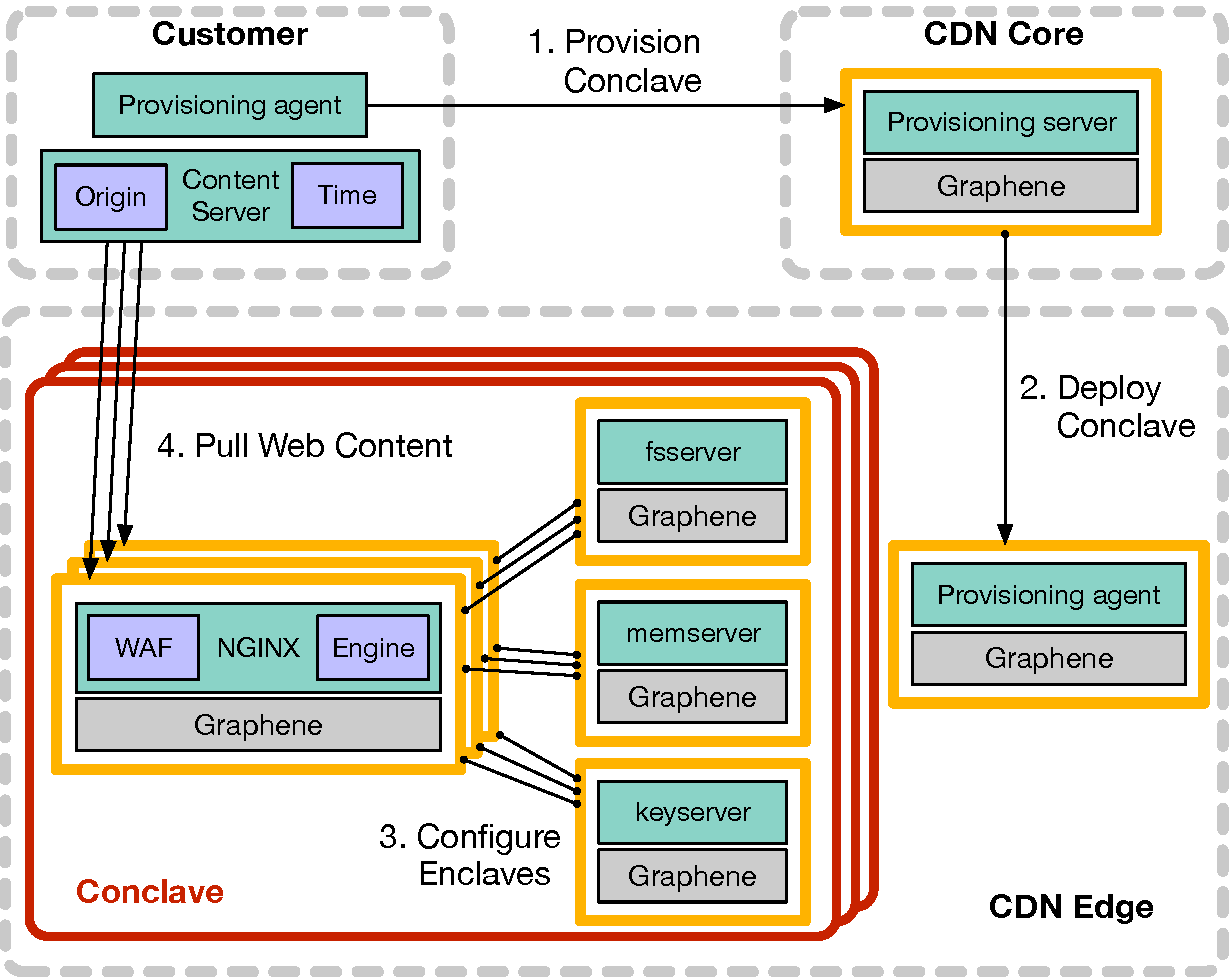
\includegraphics[width=0.48\textwidth]{figs/phoenix-design}
	\caption{Architectural design of \name. Multiple enclaves (yellow
	boxes) reside in a logical conclave (red boxes), permitting
	multiple processes and multi-tenant deployments. The CDN Edge and
	Core servers run on untrusted hosts.}
\label{fig:design}
\end{figure}

% }}}

The conclave design extends the open-source Graphene SGX libOS~\cite{graphene}
to support shared state abstractions among multiple processes.
%
Graphene~\cite{graphene} supports the critical system calls
\texttt{fork} and \texttt{exec} by automatically spawning a brand new
enclave, and performing a checkpoint-and-migration (essentially copying
the first enclave's memory pages into the second).
%
Graphene further offers some support for these separate processes
(enclaves) to communicate with one another over pipes, and implements
copy-on-write fork, signals, semaphores, message queues, and exit
notifications as RPCs over these pipes.
%
In other words, Graphene essentially turns a traditional multi-process
application into a ``distributed system'' of enclaves, along with some
basic plumbing to allow them to communicate with one another.


%% Key design challenges for libOSes include support for \texttt{fork} and
%% \texttt{exec}, and the subsequent management of shared state among the
%% processes.
%% %
%% Of the SGX-based libOSes, only Graphene supports forking, which it models as a
%% checkpoint and restore process migration.
%% %
%% In Graphene, multiple libOS instances coordinate over pipes to implement a
%% consistent, distributed POSIX abstraction, yet appear to the application as a
%% single, shared OS\@.  
%% %
%% In particular, Graphene implements copy-on-write fork, signals, semaphores,
%% message queues, and exit notifications as remote procedure calls (RPCs) over
%% these pipes.

However, two important multi-process abstractions that Graphene does not support with
confidentiality and integrity guarantees are a read-write filesystem, and
shared memory.
%
Graphene's sole filesystem, \texttt{chrootfs}, is modeled as a restricted view
of the host's filesystem.
%
%The contents of the filesystem are in plaintext; for read-only files, Graphene
%ensures the integrity of the file's contents by loading cryptographic hashes
%of the content into the enclaved libOS and verifying these hashes upon file
%reads; writable files have no integrity protections.
%
Graphene does not support shared memory at all (neither anonymous nor
file-backed).


Conclaves extend upon this prior design by leaning into the distributed
system nature of it.
%
We implement kernel services as \emph{kernel servers}; applications
act as clients, connecting to and issuing requests to kernel
services---via pipes or TLS network connections.
%
The kernel servers also run atop the libOS.
%
Our design is effectively that of a multi-server microkernel system,
similar to GNU Hurd or Mach-US, in which shared resource abstractions
are implemented as a set of enclaved daemons shared by all processes in
the system.
%% The daemons themselves also run atop the libOS\@.


\subsubsection{Conclave Kernel Servers}

Using the NGINX web server as a guide (as software representative of a
CDN edge server), we identified five key shared resources: files,
shared memory, locks/semaphores, cryptographic keys, and time.  
%
For flexibility in deployment configurations, we implement four servers
to manage these resources\footnote{Due to the common pattern of using
locks with shared memory, the memserver manages both.}:
%
We implement the fsserver, memserver, and keyserver as single-threaded,
single-process, event-driven servers that communicate with the application's
Graphene instances over a TLS-encrypted stream channel. 
%
The timeserver uses a datagram channel.
%
Each server is independent.


\parhead{fsserver}
%
For our file server, \emph{nextfs}, we extend lwext4's~\cite{lwext4} userspace
implementation of an ext2 filesystem into a networked server.
%
nextfs uses an untrusted host file as the backing store, similar to a block
device.
%
We develop three variants of this device to accommodate different security
postures, and a fourth for comparison purposes.

\vspace*{-0.5\baselineskip}
\begin{widelist}

\item 
%
\textbf{bd-std} stores data blocks in plaintext, without integrity
guarantees. This serves as a baseline in our evaluation.


\item
%
\textbf{bd-crypt} encrypts each block using AES-256 in XTS mode, the de
	facto standard for full-disk encryption~\cite{xts-ieee,xts-nist}.
%
We base each block's initialization vector on the block's ID.
%
This, too, lacks integrity guarantees, and is thus suitable only for an
	honest-but-curious attacker.


\item
%
\textbf{bd-vericrypt} adds integrity guarantees to bd-crypt, thus
	providing authenticated encryption.  It does so by maintaining a
	Merkle tree over the blocks: a leaf of the tree is an HMAC of the
	associated (encrypted) block, and an internal node the HMAC of its
	two children.
%
To keep the memory needs of the enclave small, bd-verity consults a
	serialized representation of the tree in a separate file, rather
	than use an in-memory representation.
%
The root of the Merkle tree exists both on the file and in enclave
	memory; the HMAC key exists only in enclave memory.
%
As an optimization for reducing reads and writes to the Merkle tree
	file, bd-verity maintains an in-enclave LRU-cache of the tree
	nodes.
	%
	bd-vericrypt is the appropriate choice in a Byzantine threat model.
	

\end{widelist}


\parhead{memserver}
%
We implement shared memory as filesystems that implement a
reduced set of the filesystem API\footnote{Graphene does not have a
unified filesystem and memory subsystem, and
thus \texttt{munmap} is not currently available as a filesystem operation.
}:
\texttt{open}, \texttt{close}, \texttt{mmap}, and \texttt{advlock}
(\texttt{advlock} handles both advisory locking and unlocking).
%
In our shared memory filesystems, files are called \emph{memory files}, and
either represent a pure, content-less lock, or a lock with an associated
shared memory segment.
% 
Memory files are non-persistent: they are created on the first open and
destroyed when no process holds a descriptor to the file and no process has the
associated memory segment mapped.


We implement three versions of shared memory.
%
Each stores a canonical replica of the shared memory at a known
location (either a particular server or file).
%% Each uses a scheme whereby a canonical replica of the shared memory is
%% stored at a known location.  
%
Upon locking a file, the client ``downloads" the canonical replica and updates
its internal memory maps.
%
On unlock, the client copies its replica to the canonical.
%
%Note that SGX does not provides a means for us to interpose on page accesses
%(as a page table handler would in normal Linux), and thus we must 
%interpose through the locking and unlocking system calls.
%\begin{widelist}

\vspace*{-0.5\baselineskip}
\begin{widelist}

\item 
%
\textbf{sm-vericrypt-basic} uses an enclaved server to keep the canonical
memory files in an in-enclave red-black tree.

\item 
% 
\textbf{sm-vericrypt} implements a memory file as two untrusted host files: a
mandatory lock file, and an optional segment file.
%
When a client opens a memory file, the sm-vericrypt server creates the lock file on the
untrusted host, and the Graphene client maps (\texttt{MAP\_FILE|MAP\_SHARED})
the lock file into untrusted memory.
%
The client then constructs a ticketlock structure over this untrusted shared
memory.
%
Since the untrusted host may manipulate the ticketlock's turn value, a
shadowed, trusted turn number is maintained by the enclaved sm-vericrypt
server.
%
After the client has acquired the lock, the client makes an RPC to the
server to verify the turn number.
%
The server thus acts as a trusted monitor of the untrusted monotonic
	counter.
%% As such, the server acts as a trusted, monotonic counter that monitors an
%% untrusted monotonic counter.


If a client \texttt{mmap}s the memory file, the server creates the
associated segment file on the untrusted host.
%
When the client subsequently locks the file, the client makes a \texttt{lock}
RPC to server, which returns the keying and MAC tag information for
the segment.
%
The client copies the untrusted memory segment into the enclave, and uses
AES-256-GCM to decrypt and authenticate the data.
% 
When a client unlocks the file, the client generates a new IV, copies an
encrypted version of its in-enclave memory segment into the untrusted
segment file, and makes an \texttt{unlock} RPC to the server, passing along
the new IV and MAC tag.

% \clg{I think this section can be compressed}

\item 
%    
\textbf{sm-crypt} 
	%is like sm-vericrypt, but 
	assumes the untrusted host does not
tamper with data.  As such, sm-crypt uses AES-256-CTR instead of AES-256-GCM,
and does not need an enclaved server to monitor the integrity of the ticketlock
and IV.

\end{widelist}




\parhead{keyserver}
%
The keyserver is an SGX enclave rendition of a hardware-security module
(HSM): the keyserver stores private keys and performs any private key
cryptographic operations.
%
Like Keyless SSL~\cite{keyless-ssl}, this not only maintains the
confidentiality of the private key with respect to an untrusted host,
but also isolates the key to an address space distinct from the
application's, thereby guarding against critical memory disclosure
vulnerabilities, such as Heartbleed~\cite{heartbleed-cve}.


We implement the keyserver as two components: the keyserver proper, and an
OpenSSL engine (``engine'' in Figure~\ref{fig:design}) that the application
loads as a shared library; the engine proxies private key operations to the
keyserver.
%
Unlike the fsserver and memserver clients, the key client operates at
the application layer, outside of Graphene.


OpenSSL's engine API requires the caller (in our case, NGINX) to provide an
\texttt{RSA} object, which contains the secret key.
%
To avoid having to expose the key, we modified OpenSSL to populate
\texttt{RSA} objects with dummy keys that instead serve as identifiers
that the keyserver uses to look up the real keys it stores securely.


To reduce the number of connections and avoid a dependency on the memserver for
lock files, our engine maintains the property that all keys for the same
keyserver, within the same process, share a single connection.
%
This requires that the engine detect forking by the application, which we
achieve by also associating process IDs with the \texttt{RSA} objects.


\parhead{timeserver}
%
Given that the components of a conclave must authenticate one another,
we need trusted time to guard against attacks that 
% manipulate the conclave's sense of time to
trick the conclave into accepting expired certificates.
%% (and therefore possibly
%% cracked) certificates.
%
Unfortunately, SGX itself does not provide trusted time.  
%
Its SDK~\cite{sgx-linux-sdk} provides features~\cite{sgx-trusted-time}
for retrieving coarse-grained, monotonic time through a protected clock
provided by Intel's Converged Security and Management Engine (CSME),
but not all processors support it~\cite{ayeks-sgx-hardware}.
%

%% Techniques that base wall-clock time on the \texttt{RDTSC} family of x86
%% instructions cause a \texttt{\#UD} fault in SGXv1, while in SGXv2 the
%% instruction may be modified by a hypervisor.
%% %
%% Intel's SGX SDK~\cite{sgx-linux-sdk} does provide
%% features~\cite{sgx-trusted-time} for retrieval of coarse grained, monotonic
%% time, through a protected clock provided by Intel's Converged Security and
%% Management Engine (CSME)\@.  
%% %
%% However, this feature relies on the presence of the CSME (not all processors
%% include this firmware~\cite{ayeks-sgx-hardware}), and moreover relies on an
%% enclave to securely obtain a base wall-clock time from a remote, trusted,
%% server.


Instead of relying on the CSME, we simply design a remote, signed
timestamping server.
%
The timestamping server runs outside of an enclave, on a remote trusted
machine (e.g., at the CDN's customer).
%
The timeserver's purpose is not to provide fine grained precision to
the conclaved processes, but rather to serve as an integrity check of
the time those processes receive from the untrusted host.

We modify the Graphene system call handlers for \texttt{getttimeofday},
\texttt{time}, and \texttt{clock\_gettime} to optionally proxy application
calls to a remote, trusted, timestamp signing server.
%
The use of such a timeserver, and the related parameters, such as the
timeserver's public key, are specified by the Graphene user (here, the content
provider), and hard-coded into Graphene's configuration.
%
As a freshness guarantee, each request includes a new, random
nonce, generated by the Graphene system call handlers.
%
The timeserver, in turn, returns an RSA signature over a message
consisting of the current time concatenated with this nonce.


%% As time-related system calls occur frequently in event-driven applications like
%% web servers, and as each timeserver request incurs latency due to both the
%% network and RSA operations, the Graphene client makes remote requests for  $p$
%% percent of the time-related system calls, where $p$ is a configurable
%% parameter.
%% %
%% Upon verifying a timeserver response, the Graphene client retrieves the time
%% as reported by the untrusted host, and verifies that the time the host
%% returns is within a configurable tolerance to the timeserver's time.
%% %
%% For a time-related call in which the Graphene client does not consult the
%% timeserver, Graphene checks that the time returned by the untrusted host is
%% greater than the last time value retrieved.


Our timeserver approach resembles Google's roughtime protocol~\cite{roughtime};
future work would fully port the roughtime protocol to Graphene to reduce the
need for a trusted timeserver by instead tolerating some fraction of
misbehaving servers.
%
Note, however, that, in the SGX setting, both our approach and roughtime are best
efforts; an untrusted host that identifies the traffic between the Graphene
client and timeserver could, for instance, ``slow down" time by delaying the
responses.



\subsubsection{Conclave Images} % {{{

Conclaves bundle the SGX microkernel runtime and application suite into a
deployable and executable image, reminiscent of a traditional container image.
%
When the conclave is executed, the first enclave process that is
executed is an init process, which executes the kernel servers and the
specified application proper.
%
From that point, the application can fork, spin up new applications,
and so on.


\subsubsection{Bootstrapping Trust} % {{{

%% Before we address provisioning secrets to the running conclave, we describe

We first address how the conclave, viewed as a distributed system,
establishes the trust of each member node, whether kernel server or
application process.
%
This is a chicken-and-egg problem of establishing a secure channel
between two nodes without first provisioning these nodes with, say,
private keys and certificates for mutual authentication.
%
%% 
%% 
%% %
%% There are two cases we must address: (1)~trust between a parent-child
%% relation (for instance, between the init and the processes it spawns),
%% and (2)~trust between non parent-child process relationships (such as
%% between the application nodes and the kernel servers).
%% %
%% In both cases, the problem boils down to a chicken-and-egg dilemma of
%% establishing a secure channel between two nodes without first
%% provisioning those nodes with, for instance, private keys and
%% certificates for mutual authentication.
%% %
%% If we can establish such a channel, then provisioning becomes
%% straightforward: NGINX servers can simply (and safely) read sensitive
%% key material from keyservers, and read and write sensitive user data in
%% the fsserver and memserver.



The standard approach for establishing a secure channel in an SGX setting is to use SGX
as a root of trust and enclave attestation as a form of authenticated identity,
and to merge this form of attestation into the establishment of the shared
channel secret.
%
To that end, \name follows closely from the work of Knauth et
al.~\cite{DBLP:journals/corr/abs-1801-05863}, which 
integrates attestations with TLS by adding the SGX quote as an X.509
certificate extension.
%
This has the effect of making channel establishment and SGX attestation
occur together,
atomically, with respect to the channel protocol.
%
%% prevents
%% man-in-the-middle attacks by making channel establishment and SGX
%% attestation occur together, atomically, with respect to the channel
%% protocol.
%% %
%% The core problem they address is that, to prevent
%% man-in-the-middle attacks, secure channel establishment and SGX attestation
%% must occur together, atomically, with respect to the channel protocol.
%% %
%% In order to do this, they integrate attestation with TLS by adding the SGX
%% quote as an X.509 certificate extension.
%% %
Certificate validation can thus be extended to examine these new extensions.


Adding new certificate extensions, of course, is not the full story.
%
In this setup, the enclave generates an ephemeral key pair.
%
SGX quotes are, mandatorily, over the enclave image, the enclave signer,
non-measurable state, such as the enclave mode (e.g., debug vs production),
and, optionally, any additional data (user data) the enclave wants to
associate with itself.  
%
The trick for ensuring the atomicity of attestation and secure channel
establishment is for the enclave to specify as user data a hash of the ephemeral
public key.
%
Since the key pair is created within the enclave, and since only an enclave can
get a valid quote, such user data binds the key pair to the enclave.
%
The enclave then generates a self-signed certificate for this ephemeral public
key, which includes the aforementioned extensions for the quote and IAS
verification.


In our conclave setup, the attestation is a local attestation, and validation of
the quote is based on a list of valid attestation values in the manifest.
%
Specifically, the manifest specifies a graph of which processes can establish
secure channels with one another.


\subsection{Evaluation}

Figure~\ref{fig:macrobench-single-tenant-lat-throughput} shows
request latency and throughput results for the four configurations.
%
Due to the RSA private key operation in the TLS handshake, Linux becomes
CPU-bound at four workers (our test machine has four physical cores) and
saturates the Ethernet link for tests with a 100~KiB payload and more than one
NGINX worker.
%
Linux-keyless shows that the concurrency of the keyserver levels
off with two workers, and thus that the two NGINX worker configuration of
Linux-keyless is an upper-bound on the performance we can hope to achieve
with the other conclave configurations.
%
%In addition, whereas Graphene-crypt shows increased performance as the number
%of workers increases, Graphene-vericrypt tops off at two workers, before
%showing worse performance with more NGINX workers.
%
To compete with a one worker Linux configuration, Linux-keyless needs two
workers, and Graphene-crypt needs four; Linux with two or more workers beats
all conclave configurations.


\begin{figure}[t]
	\centering
    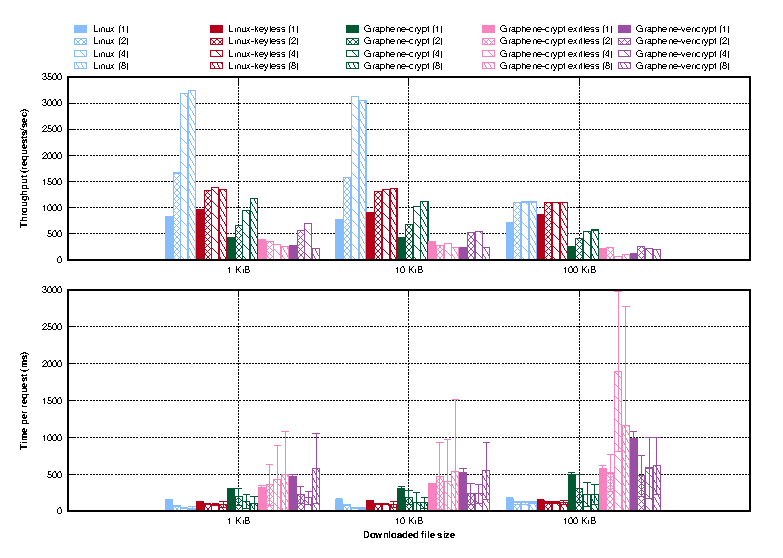
\includegraphics[width=0.5\textwidth]{figs/macrobench-single-tenant-lat-throughput}
	%
	\caption{Throughput and latency for single tenant configurations.
    The legend indicates the number of NGINX worker processes.
    We include the standard deviation of the latencies as error bars.}
	%
	\vspace*{-4pt}
    \label{fig:macrobench-single-tenant-lat-throughput}
\end{figure}

\section{Proposed Gemini Design}
\label{sec:gemini-design}
%
% 1. give a 1-2 paragraph overview of the architecture
% 2. Create a subsection for each major component of the architecture
%       2-3 paragraph overview of component
%       parheads (with 2-3 paragarphs of content) for each design
%       choice/challenge/consideration.
% I imagine each subsection will be 1-2 columns.
%
% Throughout, point back to the use-caes, and comment on how they influence the
% design.

The Gemini design consists of a security policy specification and a monitor
that enforces the policy, both of which are transparent to applications.
%
The policy itself may aggregate rules from multiple, mutually
distrustful parties.
%
A prominent feature of the policy is that it allows for private data to be pinned
to specific trust domains, such as an organization's own machine.
%
The monitor manages the migration of an application's execution between domains
as the execution attempts to access pinned data, and ensures consistency of
resources shared between them.


Gemini's core abstraction is a \emph{distributed container},
where the filesystems and memory of the container may span several
domains, with each domain potentially cloaking parts of this space from the
others.
%
Each domain runs its own instance of the monitor, with the assumption that a
domain trusts its version of the monitor, but not those of its peers.
%
In an environment with trusted boot, where parties can attest to trusted peer
monitors, a party can augment a peer's monitor so as to enforce fine-grained
IFC rules to detect incorrect behavior during an application's execution.


We describe the three major aspects of Gemini's design: (1) the monitor, (2)
migration between domains, and (3) the security policy framework.
%
% The security policies are only interesting in the case of trusted monitors;
% otherise the policies are simply "to access object X, migrate to machine Y.
%
% Thus, I would descirbe the monitor and migration first with just that simple
% policy in mind, and then use the security policy section to describe the more
% interesting policies that trusted hardware allows.


\subsection{Gemini-0}

\subsubsection{Monitors}
%
The monitor itself must simultaneously interpose on a process's execution while
also ensuring consistent policy enforcement for shared resources, such as files
and shared memory.
%
One approach is to base the design on full-system emulation.
%
However, full-system emulation is slow, as it needlessly emulates
monitored and unmonitored processes alike.
%
Moreover, previous
systems~\cite{whole-system-simulation,panorama,demand-emulation} that use this
technique in conjunction with taint tracking suffer from a lack of system
introspection, as well as the explosion of taint into kernel space.
%
Gemini's design instead takes a hybrid approach that splits the monitor between a
per-process monitor and a system monitor.



\parhead{Process monitor}
%
The process monitor is an emulator that instruments and dispatches the
application's code.
%
The emulator instruments instructions, such as
loads and stores, that propagate taint, as well as interposes on
system calls that transfer tainted data.
%
The process monitor tracks the propagation of taint in the process's
memory space using shadowed pages inaccessible to the application.
%

\parhead{System monitor}
The system monitor keeps a system-wide account of tainted resources,
ensures that processes are run in emulation mode when they have access to
tainted data, and applies policy checks over tainted data, such as when data is
emitted to the network.
%
To track taint through storage, the system monitor applies persistent
taint tags to files.
%
% Netlabel, CIPSO IETF draft
To transfer tainted buffers over the network, the system monitor embeds taint
tags in outging packets and processes tags from incoming packets.
%
In the case of untrusted boot, the policy that the system monitor enforces is
fairly simple: if a process attempts to access a page or a file pinned to
another domain, the monitor initiates a migration of execution to that domain.


\subsubsection{Execution migration}

Gemini migrates at the thread-level.
%
When a thread attempts to access a resource pinned to a target domain,
the system monitor suspends the thread, and transfers the
thread's execution to the target.
%
The thread runs on the target until it satisfies a \emph{migration condition},
and then migrates back to the source.
%
On return, the source updates the thread's context and the process's memory
space, and resumes the thread.


\parhead{Distributed Shared Memory}
%
Similar to prior systems, Gemini integrates distributed shared memory (DSM) and
virtual memory management.
%
Each domain runs a DSM manager and page server that cooperates with the VM
manager to service page faults.
%
The VM manager refers remote memory access to the DSM manager,
which in turn satifies the request using a coherence protocol with the peer
domain's page server.
%
Thus, a page fault to local memory is indistinguishable from a page fault to
remote memory.


\parhead{Distributed Filesystem}
%
Gemini maintains a consistent filesystem view among migrated and
non-migrated processes by allowing a thread's file descriptor table on the
target to proxy calls to a fileserver back on the source.
%
This has additional benefit of obviating the need to replicate or update
public files during migration.
%
Domains may pin file descriptors, such that the descriptor can only be used
in that domain.
%
Likewise, if the target thread writes tainted data to a remote descriptor, the
associated file transfers to, and becomes pinned by, the target; any processes
on source with that file open have subsequent operations on that descriptor
proxied to the target.


\parhead{Example: Loading a private key}
%
In Figure~\ref{fig:loading-key} we diagram a provider's service (source) loading
a private key pinned to the organization's machine (target).
%
We assume that the service is proprietary, and thus the provider
pins the custom portions of the software.
%
We assume that the service's cryptographic library is public, however.


In step 1, the source's monitor detects that one of the service's threads
attempts to open the cloaked key file.
%
The monitor suspends all the threads in the process, and transfers a minimal
subset of the thread's execution state to the target.
%
In step 2, the target monitor constructs a skeleton process and
restores the source's thread.
%
In restoring the thread, the target ensures that the only executable mappings
in the process correspond to the cryptographic library.
%
Likewise, during execution, the target's monitor will ensure that thread does
not create new executable mappings.


In step 3, the target resumes the thread in the process monitor's emulator,
tracking the propagation of the private key's data by adding taint tags to
the shadow table.
%
If the thread tries to access a page that the source has not yet tranferred,
the access generates a page fault.
%
The target's monitor traps such faults and redirects them to the source, which
responds with the faulted page.


When the process monitor detects a stopping condition, it notifies the
system monitor to suspend the thread and migrate back to the source machine.
%
The stopping condition is policy-specific; examples include the process
performing $n$ consecutive instructions without tainted
data, or the instruction pointer referencing source-cloaked data or code.
%
In step 4, the source's system monitor updates it's memory mappings based on
the target's exeuction, and sets page table attributes to indicate which pages
are now cloaked by the target.
%
As with the migration to the target, the source must also perform consistency
checks.
%
The source then resumes the threads.


\begin{figure}[t]
	\centering
    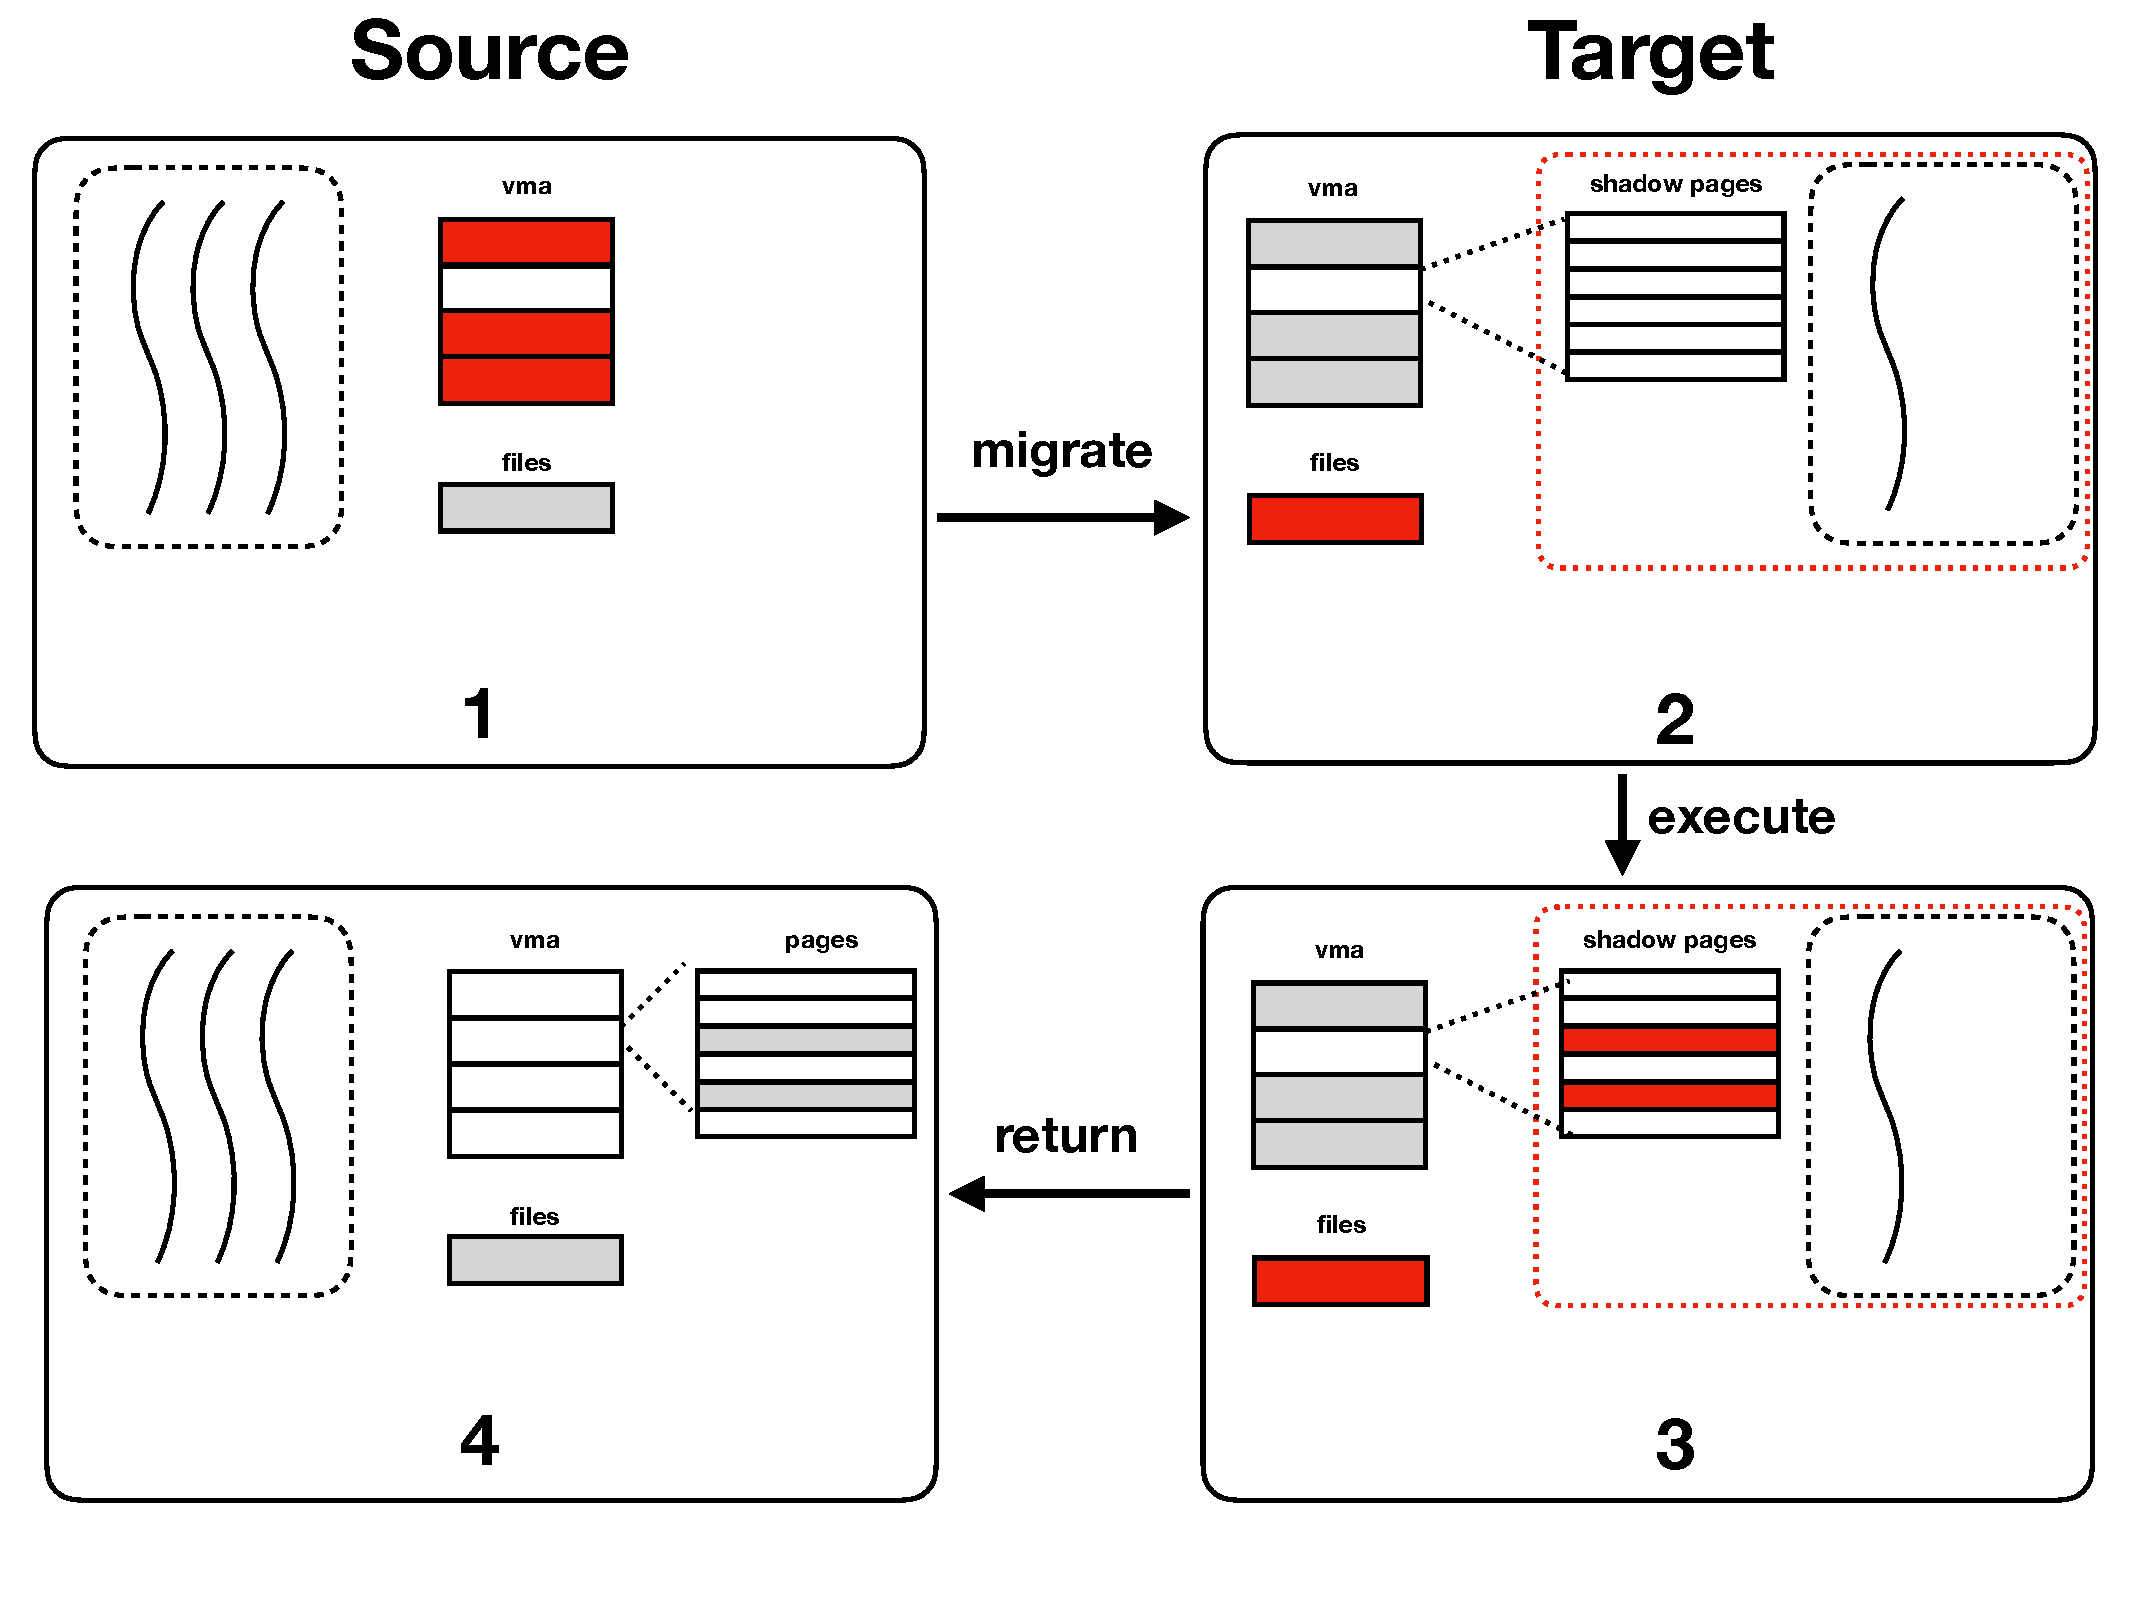
\includegraphics[width=0.5\textwidth]{figs/loading-key}
	%
    \caption{A webserver on the service provider's domain (source) loading a
    private key pinned to the organization's domain (target).
    %
    Cloaked virtual memory areas (VMAs) an files are in gray, and pinned
    resources are in red.
    }
	%
	\label{fig:loading-key}
\end{figure}


\parhead{Example: Signing operation}
%
Migration for a signing operation is similar to that for loading a
private key.
%
For signing, however, the source's monitor detects an 
access attempt to pinned data via a page fault for the cloaked memory page
storing the key.
%
When the thread, executing on the target, computes the signature, the target's
monitor must also specify a \emph{declassification gate} to remove the taint that
would otherwise pin the signature to the target.
%
In this example, the gate is a ``hook"  for the cryptographic library's
signing function.
%
With declassification gates, the target must guard against attempts by the source to
hijack declassification.
%
For instance, the source could arrange for the thread to be restored with a
starting point that invokes \texttt{sign(0, key}), thereby declassifying the key.
%
Thus, the target must properly sanitize a gate's arguments.


\parhead{Limitations}
% TODO:DSM and test-and-set?
%
A disadvantage of the integration between VM and DSM is that the unit of access
adn locking are contrainted to be a page.
%
If multiple data structures are allocated on the same page, then this constaint
can lead to \emph{false sharing}, wherein distinct private data structures
appear shared due to colocation on the same page.
%
A similar issues exists with applying taint tags at the page granularity.


Gemini is also susceptible to a form of deadlock whereby, during the course of
a thread's execution, the thread reaches an instruction that accesses two
pieces of data, each pinned to a separate domain.
%
We simply specify that Gemini must detect such occurences and abort.


In our uses-cases, this form of deadlock is either non-existent or unusual, as
only a single party has pinned data, or the pinned data of each party is used 
in logically different portions of the code (e.g., an email provider pinning
proprietary spam rules, and an organization pinning a private key).
%
A more plausible deadlock scenario is a server that supports multiple tenants
and uses a global data structure to manage the (pinned) keys across all
tenants.
%
In such cases, the application may need to be patched to correct the offending
memory layout.
%
In the general case, the problem is one of secure multi-party computation, and
an interesting area of future work is for the emulator to emit garbaled
circuits when it detects such events.


\subsection{Gemini-1}

\subsubsection{Security policies}
%
There are two types of security policies: \emph{confidentiality policies} and
\emph{integrity policies}.
%
Confidentiality policies either pin data or restrict the accesss privileges of
code with respect to the data.
%
Integrity policies specificy a service's behavior
based on the flow of the data within and from that service. 


Policies are expressed over taint tags.
%
A tag belongs to one of three classes: \emph{pinned}, \emph{provenance},
or \emph{access}.
%
A pinned tag applies to code and data, and indicates the domain (such
as a host) that has pinned the associated code or data.
%
A provenance tag applies only to data and indicates that either a domain or a piece of
code has processed that data.
%
An access tag applies to domains, code, and data, and indicates the read or
write privileges of the domain or code with respect to the data.


Organizations introduce tags into the system by either a tool (or monitor) that
tags static files, or by egress rules that tag data as it transfers from
between domains.
%
Monitors propagate the tags in accordance with computation across the memory
space, filesystem, and network.


\parhead{Confidentiality Policies}
\begin{enumerate}
    \item[C1]  The organization's private key(s) must not be leaked to untrusted parties.
\end{enumerate}


\parhead{Integrity Policies}

\begin{enumerate}
    \item[I1] If the organization's data (e.g., webpage, DNS records, emails) leaves the
        service, it must be sent over a flow endorsed by the organization's private
        key.

    \item[I2] Any flow endorsed by the organization's private key must only send
        data originating from the organization.

    \item[I3] If the organization's data leaves the service, it must not have been
        modified.
\end{enumerate}

Policies (I2) and (I3) are impractically strict: web and mail servers will add
headers to the outgoing content, and may further modify the content through a
legitimate transformation, such as compression or image transcoding.
%
Thus, these assertions may give rise to additional qualificaitons.
%
For instance, to allow for server-provided headers, assertion (3) may instead
be specified as: ``Any flow endorsed by the organization's private key must
\emph{eventually} send data originating from the organization."


\parhead{Transitive Closure Policy}

\begin{enumerate}
    \item In the case of a distributed service, the organization's data can
        traverse other nodes that  guarantee the above properties.
\end{enumerate}


% The TLS frames will contain metadata fields (sequence numbers, etc.),
% that are not tagged as belonging to the organization.
% %
% Thus, the monitor uses an application-layer parser to parse the
% messages, and consults with the policy regarding which tags should be on
% which fields.
% %
% If simple temporal logic is fine (not labeled until labeled), then the monitor
% does need the underlying plaintext; otherwise, the monitor must further impose
% an implementation requirements on the application; namely, the use of
% kernel-TLS\@.


\parhead{Example: HTTPS Edge Server}
%
Execution migrates to the organization, which produces an RSA signature, and
then execution migrates back to the CDN\@.
%
Before migrating back to the CDN, the organization assigns a taint tag to the
signature, which is also sent to the CDN\@.
%
The CDN sends the signature to a web client as part of the ServerHello TLS
message.
%
When the CDN's monitor sends the signature, it marks the corresponding flow
with the tag.


If the client requests a web page that is not in the server's cache, the server
makes an HTTPS request to the organization's origin server and downloads the
page.
%
The CDN's monitor detects that the request is made to the origin and tags the
downloaded page to indicate its provenance (alternatively, the origin server
could embed these tags in its response packets).
%
When the CDN sends the page to the client over subsequent TLS frames the
monitor checks that these frames include data that is tagged as originating
from the organization. 


\begin{figure}[t]
	\centering
    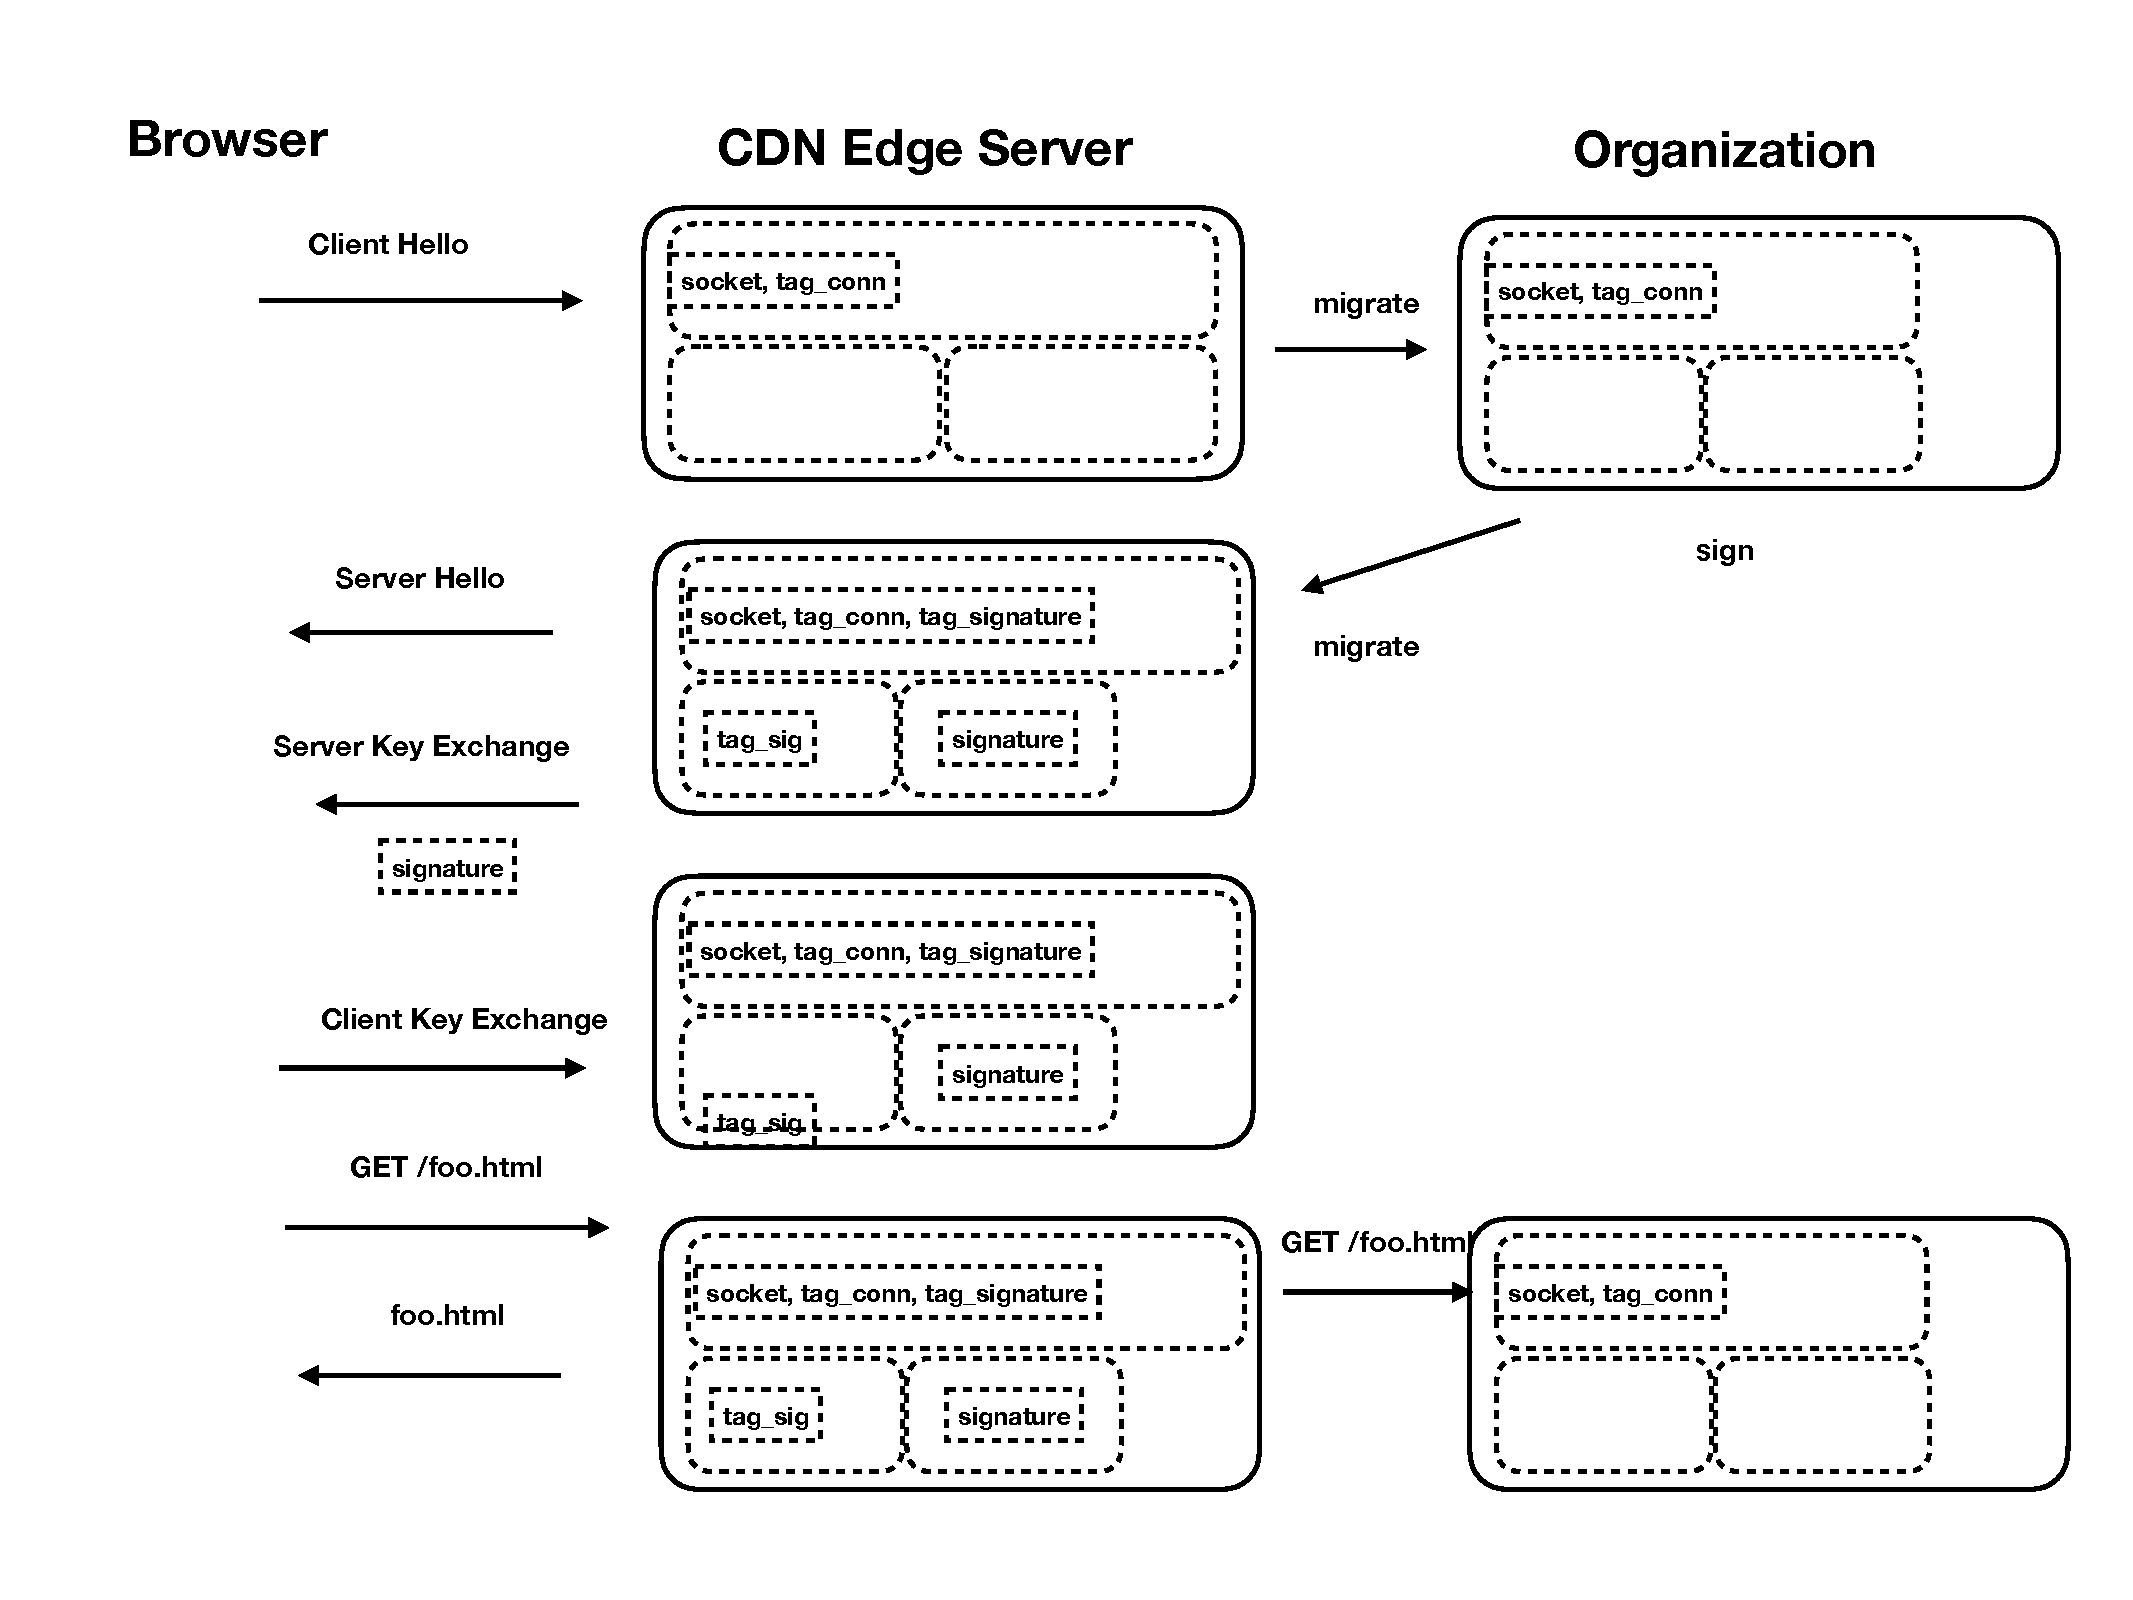
\includegraphics[width=0.5\textwidth]{figs/https-flowchart}
	%
    \caption{The evalution of taint-based firewall rules for an HTTPS proxy
    service.}
	%
	\label{fig:https-flowchart}
\end{figure}


% \parhead{Application: DNS Authoritative Server}
% %
% The firewall rules for a DNSSEC-enabled server inspects incoming packets, and keep a
% running mapping of the requests's ID to whether the request requires DNSSEC
% (the request's \texttt{DO} bit).
% %
% When sending responses, the policy  parses the response's ID and retrieves the
% corresponding \texttt{DO} value from the mapping.
% %
% If the mapping indicates that the request set \texttt{DO}, the firewall
% verifies that the response includes an \texttt{RRSIG} record tagged with the
% organization's private key.
% %
% Regardless, the firewall verfiies that the remaining response data is tagged as originating
% from the organization.


\parhead{Tag Properties}
%
\begin{widelist}
\item \textbf{Unforgeable:}
    %
    A possible attack is that the provider adds its own policy that taints data as
    if it came from the organization, and so the data passes the organization's
    policy monitor.
    %
    This threat implies that either the monitors maintain the secrecy of the tags
    from the untrusted applications, or make them unforgeable.
    %
    The problem with maintaining tag secrecy is that tags may appear as metadata
    attached to files and stream.

\item \textbf{Irrevocable:}
    %
    If Gemini is running in a secure enclave, organization $A$ might apply
    a tag to its enclaved private key that specifies that only a specific
    piece of code is allowed to access the data.
    %
    Thus, it is necessary that organization $B$ be unable to remove $A$'s tag,
    lest $B$ gain access to $A$'s private key.
    %
    In short, only an organization can remove its own tags.

\item \textbf{Multiple tags per byte:}
    %
    As shown by the two examples above, there is need for the system to support
    assigning multiple tags to a given byte.

\item \textbf{Multiple tags per organization:}
    %
    As shown by the two examples above, there is need for the system to support
    assigning multiple tags from the same organization.

\item \textbf{Large tag space:}
    %
    Due to an HTTPS or DNS server simultaneously hosting many tenants, the
    system most support a large tag space.
\end{widelist}

For space considerations, there may also be the need to perform tag coalescing, as where
many contiguous bytes share the same tag set.


\parhead{Egress Monitor}
%
Egress monitors are primarily for integrity, not confidentiality, and thus
we do not have to be concerned with the monitor laundering taint.
%
Egress monitors perform two tasks: (1) request attestations from remote
monitors, and (2) provide a mechanisms for stateful, tag-aware, packet filters.
%
One challenge is that the packet filters may have to operate over encrypted
data, which might diffuse the taint applied to the underlying plaintext.
%
In such cases, I  envision the monitor must imposing
an implementation requirement on the application; namely, the use of
kernel-TLS\@.
%
An additiona design contraint regarding performance is that, in the case of
multi-tenancy, a system may have many egress policies that are identical with
the exception of the tag values.  Thus, I might have a monitor-level policy
whereby monitors can only view data that includes one of its tags.




% How does tagging code work?
%   You could tag openssl with the a tag from the org that grants openssl
%   permission.
%
%   You could assume that openssl is tagged by openssl's org, and the data's
%   tag specifiies who can read it.
%
%   These seem pretty much the same to me.
%
%       You don't want to have to run the origin server under emulation --
%       it's not doing any taint tracking.  So, instead, you can imagine 
%       applying the taint at the network filter.
%

\section{Proposed Gemini Evaluation}
\label{sec:gemini-eval}
% Short intro that covers the gist: correctness and performance concerns.
%
% each subsection a question.  One or two paragraphs that expound upon the
% question and point to an evaluation method/tool.


\subsection{Correctness}
%
I need to ensure that a process running on Gemini shows the correct behavior
(program correctness), the isolation of pinned data (security correctness), and
the accuracy of the firewall rules (again, security correctness).
%
Pragmatically, this amounts to writing unit tests.
%
Additionally, it may involve showing generality by, for instance, instrumenting
more than just OpenSSL (the macro-benchmarks can also help to show generality
at the application-level).
%
For demonstrating data isolation, you might have an external program that just
dumps and scans a process's memory for a given byte string.


% TODO: try to think of a few correctness conditions, and what the unit test
% would look like for each one.  You might also consider tests for different
% application models, such as a single-threaded vs multi-threaded, vs
% multi-process application.


\parhead{Fault-injection tests}
%
TODO: purposefully try to send packets that do not pass the tag-aware packet
filters and verify that the filters prevent the transmission.


\subsection{Performance}

\subsubsection{Micro-benchmarks}

\parhead{How precise is taint-tracking?}
% - how do you know that taint tracking is being performed correctly
%   (not overtaintint, not undertainting).
% - eval at the call graph level 
%   take eleos annoations as hints --
%
Taint-tracking implementations may be susceptible to over-tainting or
under-tainting.
%
We develop a profiling tool that logs the functions that operate on
tainted data, and from these logs construct the call-graph the target machine
evaluates.
%
We use this tool to collect the call-graphs for migrations that compute a
signature
%
We compare this call-graph to the call-graph induced by prior manual or
static-analysis-based partitioning schemes applied to OpenSSL\@.
%
We also evaluate whether the call graph is stable across migrations.


\parhead{What is the overhead of migration?}
% The idea is:
%   - understand the mechanics of migration and "profile" each of its steps.
%       - this might point out certain optimizations
%   - compare to alterntavies
%       - to understand tradeoffs/overheads compared to alternatives
%
Suppose a thread migrates to a target machine that has pinned a private key in
order to compute a signature with that key.
%
At the network level, how would a packet capture of the migration compare to
that of an alternative RPC-based implementation, such as keyless SSL\@?
%
In particular, how much traffic and how many round-trips does migration incur,
what is the purpose of each round-trip, and what is the corresponding ratio of
goodput to throughput?
%
Moreover, is each migration identical?


Closely related to the previous question, we seek to measure the latency of
migration and the related operations.
%
Direct overhead costs include network latency, while indirect costs include the
operations of checkpointing and restoring threads, as well as any TCP queuing
delays incurred by the source machine while its threads are paused, waiting for
the migration to return.


\parhead{How much time does the application spend on each machine?}
%
Since the use-cases involve an organization outsourcing an application to a
service provider, it would defeat the purpose if the application spent the
majority of the time on organization's machine.
%
Note that ``time" may not be the correct metric.


\parhead{What is the overhead of taint tracking and policy enforcement?}

We evalute the overhead of the monitor performing taint tracking on some common
set of benchmarks (e.g., SPEC), adjusting the amount of data that is tainted.


\subsubsection{Macro-benchmarks}

% nginx: apachebench
% bind, knot DNS, nds: dnsperf
% exim, postfix, qmail, sendmail: smtp-source
%
Give our use-cases of an HTTPS, DNS, and mail server, we stress test an
implementation of each server running in a standard Linux environment, and
compare request throughput and latency to the server running on top of Gemini.
%
Specifically we stress test the NGINX webserver using ApacheBench, the BIND DNS
server using \texttt{dnsperf}, and the postfix mail server using
\texttt{smtp-source}.


For each server, we benchmark several deployment scenarios.
%
In particular, does the deployment have only the organization pinning data (one
or more private keys), or does the service provider itself also pin data (such
as a spam or web application firewall rules).
%
In the former case, only the organization runs a process-monitor.


Furthermore, does the service support only one organization, or multiple?
%
For instance, the NGINX webserver can virtually host many sites, and thus,
under Gemini, could migrate to different organizations based on the request.
%
The application server might also support different server models, such as
multi-process or multi-threaded.
%
In a multi-process, multi-tenant configuration of NGINX, each worker process
is single-threaded and could migrate to a different organization
simultaneously, whereas in a multi-threaded configuration, only a single thread
could migrate away from the service provider any time.


Additionally, what is the granularity of the firewall rules each organization
installs on the service provider's Gemini instance?
%
Are there no firewall rules, and Gemini is used purely for migration?
%
Are the firewalls simply inspecting taint at the protocol-field level, or
performing deep packet inspection, and using an in-kernel
implementation of TLS to inspect encrypted packets. 



% TODO: How is each server's evaluation different from one another?
% That is, are you able to evaluate something on a mail server that you aren't
% able to evalute on a webserver?

\section{Mixing Gemini and Conclaves}
\label{sec:mixing}

It may be possible to mix Gemini and conclaves for performance gains or
deployment flexibility. 
%
By mixing, I am referring to composition (nesting the two execution
environments), splitting (transfering between the two environments), and
combintations thereof.

\begin{widelist}
\item \textbf{Enclaves(Gemini(app))} 
    %
    A nested execution environment where Gemini runs on top of an enclaved
    operating system.
    %
    This is likely an optimization in that organizaitons may provision private
    data to the environment, rather than rely on Gemini's execution migration.  
    %
    As opposed to just enclaves, this solution has the benefits of constraining
    malicious behavior of untrusted applications via Gemini's integrity
    policies.
    %
    This solution is likely more applicable to AMD-SEV as opposed to Intel SGX
    enclaves.

\item \textbf{Gemini(Enclaves(app))} 
    %
    A nested execution environment where Gemini manages a collection of
    enclaves: Gemini enforces information flow rules amongst the enclaves and
    also enforces integrity policies on the data flows.
    %
    This solution is likely more applicable to an Intel SGX as opposed to
    AMD-SEV enclaves.


\item \textbf{Gemini(app) + Enclaves(app)):}
    %
    A split execution environment where the application migrates between the
    two enviroments (or between compositions of the two environments).
    %
    For instance, under Gemini, a could process locally migrated into an Intel
    SGX enclave.
    %
    This is likely an optimization over a simple composition of the two
    environments.
    

    There is also a picojump-inspired use-case of moving sensitive code to data.
    %
    This use-case assumes that the data is too voluminous to transfer.
    %
    If the data is non-sensitive, no further work is needed; if the data is
    sensitive, then the data machine may require that taint-tracking run within
    the enclave, and apply egress filters on the the return migration.
    %
    This assumes that the enclaved process will not launder taint.
\end{widelist}

\section{\emph{Para} Techniques for Conclaves and Gemini}
\label{sec:para}

TODO: If a developer knows that his applications is running in such an
environment, are there any design choices a developer can make for, say, better
performance or more flexible configurations?  Is this just a case of applying
good engineering wrt to modularization and encapsulation, or are there any
deeper insights?  Usually, the efficienty of these solutions comes from
avoiding needless context switches.  So, with Gemini, you would look to hints
that could prevent needless migrations or deadlock.  This might just be memory
allocators.  Additionally, since the policy monitors have to decode the data
(tls, parse), you might be able to have the application avoid some of this.


\section{Conclusion}
\label{sec:conclusion}
% restate: 
%   - problem
%   - work you have done to solve this
%   - work you propose
%   - what success means

In this proposal, I discuss the problem of running applications that
assume a monolithic trust setting under conditions where that assumption no
longer holds, as due to a multi-party deployment or input data.
%
I posit that a major difficulty in solving this problem is the lack of support
that operating systems and programming languages offer for expressing
computation over an execution model that involves heterogeneous trust.
%
My approach is to apply operating system designs and fine-grained information
flow control techniques to hoist, or otherwise partition, the execution
environment into trust boundaries, thereby making the details of moving the
execution between trust domains, and restricting information flow among domains, a
concern of the run-time execution environment, rather than the application
developer.
% 
A primary goal of this approach is to keep the changes to the execution environment
transparent to the applications, such that these techniques allow for
\emph{post-hoc} refinements of a legacy application's trust model.
% 
I describe my prior work of enhancing library operating system for Intel SGX
enclaves,and propose codomains, an execution model that allows an application to
dynamically switch execution to different domains.
%
If successful, I will enable application deployment options that preserve
the privacy of the involved parties, as well as support the development of
applications that securely leverage the collective value of private data sets.


\bibliography{confs_long,main}
\bibliographystyle{acm}
\end{document}
